\chapter{Coplanar waveguide}
\section{\label{sec:Coplanar Waveguide Design}Coplanar waveguide design}
Week of 01/10/2018

\noindent This section investigates the quality factor, $Q$ of a coplanar waveguide (CPW) resonator up to the maximum Nb film thickness, $d$ of 300 nm. The temperature regime (~4 $K$) of operation results in the loss being dominated by interactions between thermal quasi-particles.      

\subsection{CPW basics}

\noindent The CPW resonator consists of a center conductor surrounded by ground planes fabricated using the method of optical lithography onto a substrate. There are options of different geometries of capacitively coupled CPW resonators as shown in Fig.~\ref{fig:CPWgoppl08}(a). The conductor coupling enables transmission of input and output signals.

\begin{figure}[h]
\centering
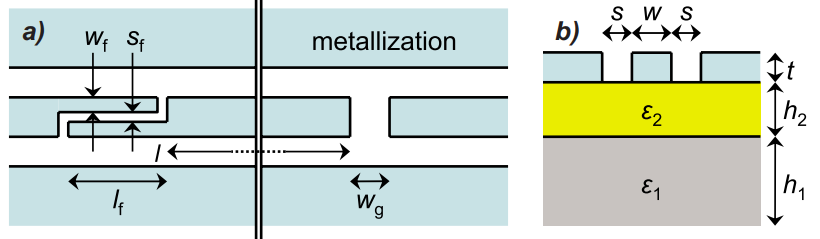
\includegraphics[height=0.3\textwidth,keepaspectratio]{CPWgoppl08}
\caption{\label{fig:CPWgoppl08} (a) CPW top view with finger capacitors (left) and gap capacitors (right). (b) CPW design cross section with a double layer substrate (yellow and grey)~\citep{doi:10.1063/1.3010859}.}
\end{figure}

The CPW cross-sectional view is shown in Fig.~\ref{fig:CPWgoppl08}(b) where the metal thickness is denoted by $t$ is most often referred to in the literature as $d$, therefore I will use the more conventional descriptor $d$. The central conductor width $W$ and the gap between the conductor and ground plane $S$ are values which impact the geometric inductance and capacitance. The capacitance and inductance per unit length are given as:

  

\subsection{CPW Q factor}
The quality factor describes how underdamped (high $Q$) or overdamped (low $Q$) a resonator is. The loaded quality factor is a parallel combination of internal and external (capacitive coupling) quality factors. The model for a LCR resonator quality factor utilised for derivation for the CPW by Yoshida in Ref.~\citep{402973}. The LCR resonator $Q= \frac{\omega L}{R}$ can be derived from considering that $Q$ is ratio of the total energy stored to the total energy lost per cycle\footnote{Useful link: http://www.techlib.com/reference/q.htm}. 

The lump inductance of the CPW is given as $L_{l} = L_{g}+L_{k}$ where 
An expression for the kinetic inductance per unit length, $L_{k}$ term only appears when the conductor is superconducting. The following inductance expressions where derived using conformal mapping in Ref~\citep{1347-4065-33-10R-5708} and Ref.~\citep{402973} based on a number of assumptions for a NbN film. (1) The wavelength of the transmitted wave is much greater than $W$. (2)  the magnetic field outside the film acts as a perfect conductor. (3) $d < 2 \lambda_{L}$ where $\lambda_{L}=\sqrt{\frac{m_{e}}{\mu_{0} n_{e}q_{e}}}$  is the London (magnetic) penetration depth which characterizes the distance to which a magnetic field penetrates into a superconductor till it becomes equal to $\exp(-1)$ times that of the magnetic field at the surface of the superconductor. (4) Uniform current density into the film. 

The results for the geometric inductance $L_{g}$ and $L_{k}$ are given as:
 \begin{equation}
\label{eq:geometricinductance}
L_{g} = \frac{\mu_{0}}{4}\frac{K(k')}{K(k)},
\end{equation}
\begin{equation}
\label{eq:kineticcapacitance}
L_{k} = \mu_{0}\frac{\lambda}{dW} g(S,W,d),
\end{equation} 
\noindent where $K(k)$ is the complete elliptic integral of the first kind with modulus $k = W /(W + 2S)$ and $k'=(1-k^{2})^{1/2}$. The geometrical factor $g(S , W, d)$ is:
\begin{equation}
\label{eq:geometricfactor}
g(S,W,d) = \frac{1}{2k^{2}K(k)^{2}} \left [ \left ( -\ln{\frac{d}{4 W}}-\frac{W}{W+2S} \right ) \ln{\frac{d}{4(W+2S)}} + \frac{2(W+S)}{W+2S} \ln{\frac{S}{W+S}} \right ]
\end{equation}
\noindent which is not sensitive to changes in $d$ and $S$ such that $L_{k}$ increases as $d$ or $S$ decrease.  Additionally for $d < \lambda_{L}$, $L_{k}$ dominates $L_{l}$. 
 
 Investigation of $L_{k}$ is completed by measuring the temperature of dependence of the resonant frequency given as:   
 
\begin{equation}
\label{eq:tempresonantfrequency}
f_{c}=\frac{1}{2 l_{r} \sqrt{L(t)C}},
\end{equation}

\noindent where $t = T/T_{c}$. Therefore the lump inductance per unit length $L_{l}(t)$ is given as: 
\begin{equation}
\label{eq:templumpinductance}
L_{l}(t)=L_{g}+L_{k}(0) \theta_{k}(t),
\end{equation}
\noindent where the small temperature dependence of $L_{g}$ (for a thin electrode the magnetic field penetrates through) is neglected. The temperature dependence of $L_{g}$ is represented by $\theta_{k}(t)$ where the assumption is that  $\theta_{k} (t) \approx \theta_{\lambda_{L}} (t) ^{2}$ since from Eq.~\ref{eq:kineticcapacitance} is can be determined that $L_{k} \propto \sqrt{\lambda_{L}}$. Additionally  $\theta_{\lambda_{L}} (t)$ is provides the temperature dependence of the London penetration depth such that $\lambda_{L}(t) = \lambda_{L}(0) \theta_{\lambda}(t)$. Good experimental agreement to the experimental value calculated using Eq.~\ref{eq:kineticcapacitance} is achieved for the approximated expression:
\begin{equation}
\label{eq:tempLondonpentration}
\lambda_{L}(0) = 1.05 \times 10^{-3}\sqrt{\frac{\rho(T_{c})}{T_{c}}}m,
\end{equation} 

\noindent where $\rho(T_{c})$ is the normal state resistivity at $T=T_{c}=4.2$ K.

The $\theta_{\lambda_{L}}$function of NbN is approximated using the local limit BCS theory since $\lambda_{L}/\xi>> 1 $, where $\xi$ is the coherence length. Superconducting CPW devices were fabricated on a Si substrate where $d$ ranging between 100-400 nm and $W$ between 40-120 $\mu$m. The half wavelength resonator is built in and the CPW is coupled at both ends to connection lines such that the resonance frequency is measured as the temperature is swept. In the low temperature regime $f_{c}$ is constant and decreases rapidly as $T \rightarrow T_{c}$. 

Fig.~\ref{fig:LkvsT} provides comparison of the theoretical and experimentally determined $L_{k}(0)$ which is expressed as $L_{k}(0)/\lambda_{L}(0)^{2}$ to provide independence of the sample $\lambda_{L}$. 

\begin{figure}[h]
\centering
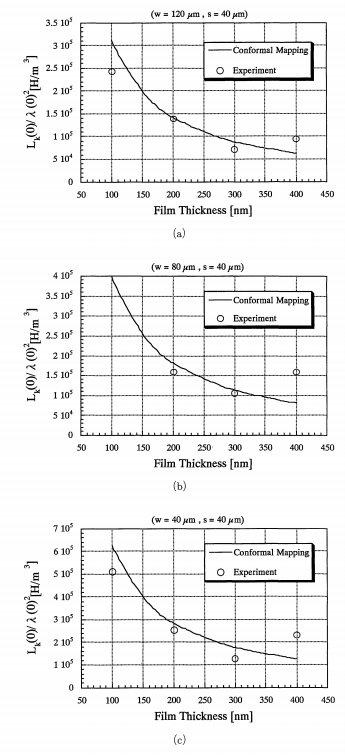
\includegraphics[height=1\textwidth,keepaspectratio]{LkvsT}
\caption{\label{fig:LkvsT} $d$ dependence of the $L_{k}$ of NbN CPW resonator for (a) $W$=120 $\mu$m (b) $W$= 80 $\mu$m and (c) $W$=40 $\mu$m \citep{1347-4065-33-10R-5708}}
\end{figure}

In Ref.~\citep{402973} an expression for the resistance per unit length is given as:

\begin{equation}
\label{eq:reistanceperunitlength}
R = \frac{\sigma_{1}}{\sigma_{2}} W L_{k}
\end{equation} 
where $\sigma= \sigma_{1}-i\sigma_{2}$ is the complex conductivity. 

  
In local limit BCS theory the temperature dependence of $\lambda$ is:

$\theta_{\lambda} (t) = \lambda (T)/ \lambda (0) = 1 / \sqrt{\frac{1}{\Delta (t)} \frac{d(\Delta (t)/t)}{d(1/t)}}$

2$\Delta$ is the energy gap 


In order to be independent of the penetration
depth of each sample, we plotted the kinetic inductance
divided by square of the magnetic penetration depth given by
(7) as a function of the film thickness.

The capacitance and inductance based on the geometry of the CPW are calculated using conformal mapping techniques 


\begin{equation}
\label{eq:geometriccapacitance}
C_{g}=4\epsilon_{0}\epsilon_{eff}\frac{K(k_{0})}{K(ko')}
\end{equation}








total inductance is calculated as the sum of the internal resonator inductance $L_{g}$ and the kinetic inductance $L_{k}$ which are given as: 




The aim is to achieve a $Q$ which is quasi-particles limited:

\begin{equation}
\label{eq:Qquasilimited}
Q_{qp} = \frac{\sigma_{2}}{\sigma_{1}} \left ( 1 + \frac{L_{g}}{L_{k}} \right )
\end{equation} 



\noindent This expression is derived from 

\begin{equation}
\label{eq:quasilimited1}
\frac{\omega_{c}}{(L_{k}+L_{L_{g}})}{Rs}
\end{equation}


